\documentclass[11pt, a4paper]{article} % setsfont size and layout

%% required packages %%

\usepackage[margin=2.5cm]{geometry} % margins
\usepackage[utf8]{inputenc} % Umlaute
\usepackage{amsmath,amssymb}		% math formulas
\usepackage{graphicx}		% graphics
\usepackage{fancyhdr}		% header and footer on every page
\usepackage{setspace}		% line space (e.g. \singlespacing, \onehalfspacing or \doublespacing)

\usepackage{braket}
\usepackage{xcolor}
%% Here the main part of the document begins %%

\begin{document}
	
%% Some more settings %%
	
\setlength{\parindent}{0pt} % first line in paragraph will not be indented
\onehalfspacing				% 1.5 line spacing
%\thispagestyle{empty}		% no header and page number on first page


%% Header on first page with course information etc. %%
\begin{tabular}{p{15.5cm}}
	{\large \textbf{Classical Mechanics}} \\
	Westlake University \\ 
	\hline
	\\
\end{tabular}

\vspace*{0.1cm}				% vertical space between header on top of the page and main heading


%\begin{center}
%	{\Large \textbf{Final Exam}}
%	\vspace{2mm}
%Name: 
%\end{center} 
%\vspace{0.1cm}
\large \textbf{Total Points: 160 points}\\
{\bf \color{red} Deadline: 9:00 pm, September 22nd, 2025} \\
{\color{blue} All problem sets and your solutions must be kept private. Please do not share them publicly or with future students. All answers must be \textbf{handwritten}, then scanned or photographed, and submitted via Canvas. } 

\section*{A particle in two dimensions attached to a spring [20 points]} 
A block of mass $m$ is free to move on a frictionless tabletop under the influence of an attractive Hooke's-law spring force $F=-k\textbf{r}$, where the vector $\textbf{r}$ is the position vector of the particle measured from the origin. Please derive the motion $x(t)$, $y(t)$ of the ball and show that the angular momentum of the ball about the origin is conserved.

\begin{figure}[h]
    \centering
    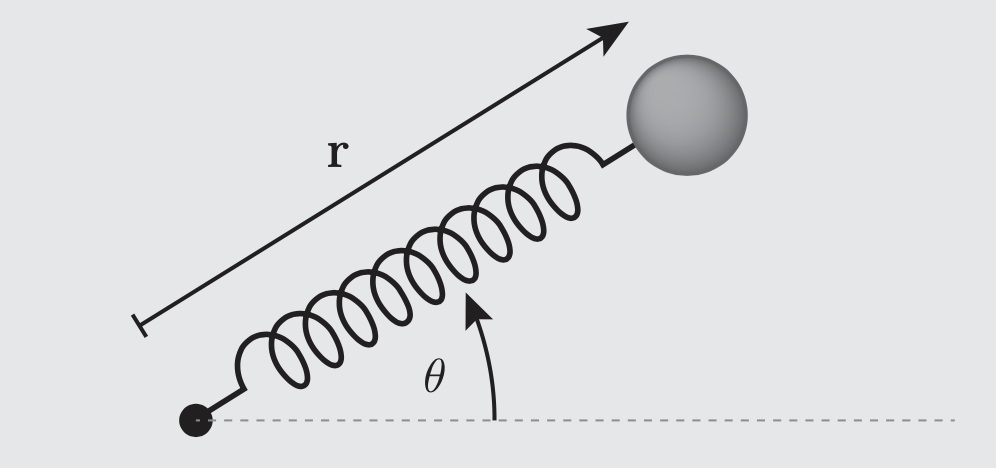
\includegraphics[width=0.5\textwidth]{PS1_P2.png}
    \label{P2}
\end{figure}

\newpage
\section*{Projectile with drag [15 points]} 
Consider a projectile subject to a drag force $\textbf{F}=-m\alpha \textbf{v}$. If it is fired
with speed $v_0$ at an angle $\theta$, it can be shown that the height as a function of time is given by 
\begin{equation}
    y(t) = \frac{1}{\alpha} \left( v_0 \sin \theta + \frac{g}{\alpha} \right) \left( 1 - e^{-\alpha t} \right) - \frac{g t}{\alpha}.
\end{equation}
Show that this reduces to the usual projectile expression $y(t)=v_0(\sin\theta) t - gt^2/2$. What exactly is meant by ``small $\alpha$"? \\
Bonus question [5 points]: Derive Equation (1) using Newton's second law. 

\newpage 
\section*{Potential energies for positive power-law forces [15 points]} 
A particle moves in one dimension subject to the power-law force $F=-kx^n$, where the coefficient $k$ is positive, and $n$ is a positive integer. Please find the potential energy of the particle and also the maximum distance $x_{\rm max}$ it can reach from the origin, in terms of its maximum speed $v_{\rm max}$. The maximum distance is the \textbf{turning point} of the particle, because as the particle approaches this position it slows down, stops at $x_{\rm max}$, and turns around and heads in the opposite direction.

\newpage 
\section*{Problems from Classical Mechanics of John R. Taylor [110 points]} 
Chapter 1: 1.27, 1.46, 1.37, 1.47 [10$\times3$ + 15 points]\\
Chapter 4: 4.2, 4.3, 4.21, 4.23, 4.27, 4.25 [$10\times5$ + 15 points]\\


\end{document}